\section{Design requirements}

Houben et al.'s proposed device shown on figure \ref{fig:old-hypr} was taken as a reference, with regards to weight, thickness and size. Although the new design retains the same purpose, the feature of having a dock for a tablet was removed, to further reduce the size. The hybrid patient record was then re-imagined to be just a thin support for a folder, with electronics on the back. \\

Working from Houben et al.'s proposed device, a new set of requirements have been established, in order to improve on the design. The following is a list of requirements pertaining to the new device:

\begin{itemize} \itemsep0em
	\item Weight: less than 500g
	\item Thickness: less than 20mm
	\item Size: Approximately same dimensions as A4 paper
	\item Maintainability: easy access to the microcontroller's programming interface
	\item Maintainability: easily change components without changing physical design
\end{itemize}

A set of requirements pertaining to the electronic part of the device has also been decided:

\begin{itemize} \itemsep0em
	\item Rechargeable battery via standard USB cable
	\item Battery status LEDs
	\item Autonomy of at least 8 hours on battery, with normal use
	\item LEDs showing colour combinations should be easily seen and understood from 10m 
	\item Hear the audio signal in a room, when device is under bed sheets
\end{itemize}

\begin{figure}[h]
\begin{center}
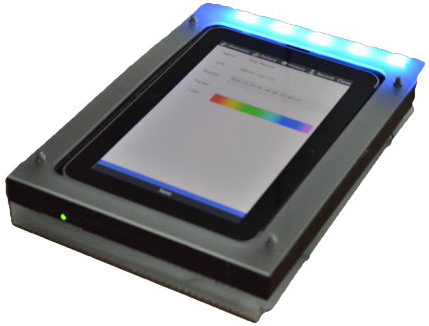
\includegraphics[scale=.5]{figures/old-hypr.jpg}
\caption{\small {\it {This is a description}}} \label{fig:old-hypr}
\end{center}
\end{figure}